\documentclass[10pt,a4paper]{amsart}
\usepackage{amsmath,amssymb,amsthm,graphicx}
\usepackage{hyperref}
\usepackage{tikz}
\usepackage[all]{xy}

\usetikzlibrary{arrows.meta}

\usetikzlibrary{shapes.misc}
\usetikzlibrary{decorations.pathmorphing}

\usepackage{euscript}


\DeclareMathOperator{\Aut}{Aut}
\DeclareMathOperator{\Bir}{Bir}
\DeclareMathOperator{\Auteq}{Auteq}
\DeclareMathOperator{\Ext}{Ext}
\DeclareMathOperator{\Quad}{Quad}

\def\CH{\mathrm{CH}}
\newcommand {\Coh} {\operatorname{Coh}}
\newcommand {\ccoh} {\operatorname{coh}}
\def\etaX{\eta}
\def\bc{\mathrm{bc}}
\def\ls{\mathrm{ls}}


\newcommand{\Sch}{\mathrm{Sch}}
\newcommand{\Sets}{\mathrm{Sets}}
\newcommand{\Spec}{\mathrm{Spec}}
\newcommand{\Sym}{\mathrm{Sym}}
\newcommand{\Cob}{\mathrm{Cob}}
\newcommand{\Sph}{\mathrm{Sph}}
\newcommand{\Ham}{\mathrm{Ham}}
\newcommand{\FS}{\mathrm{FS}}
\newcommand{\std}{\mathrm{std}}
\newcommand{\Bl}{\mathrm{Bl}}
\newcommand{\Adm}{\mathrm{Adm}}

\newcommand{\st}{\mathrm{st}}
\newcommand{\ct}{\mathrm{ct}}
\newcommand{\Tw}{\mathrm{Tw}}
%\newcommand{\tw}{\mathrm{tw}}
\def\BC{\mathrm{BC}}
\def\LS{\mathrm{LS}}
\def\bimod{\text{-mod-}}
\def\lmod{\text{-mod}}
\def\rmod{\text{mod-}}
\def\yon{\mathcal{Y}}
\def\specm{\mathsf{Spec}_\fm}
\def\fm{\mathfrak{m}}
\def\d{\mathbf{d}}

\newcommand{\scrM}{\EuScript{M}}
\def\scrA{\EuScript{A}}
\def\scrJ{\EuScript{J}}

\def\scrK{\EuScript{K}}

\def\scrP{\EuScript{P}}
\def\scrQ{\EuScript{Q}}
\def\scrR{\EuScript{R}}
\def\scrN{\EuScript{N}}
\def\cL{\EuScript{L}}
\def\cO{\EuScript{O}}
\def\cT{\EuScript{T}}
\newcommand{\scrF}{\EuScript{F}}
\newcommand{\scrC}{\EuScript{C}}
\newcommand{\scrE}{\EuScript{E}}
\def\scrW{\EuScript{W}}
\def\scrHom{\mathcal{H}om}
\def\scrV{\EuScript{V}}

\DeclareMathOperator{\Diff}{Diff}

%\DeclareMathOperator{\Bir}{Bir}
\DeclareMathOperator{\Symp}{Symp}
\DeclareMathOperator{\Stab}{Stab}
\def\P{\mathcal{P}}
\newcommand{\NS}{\operatorname{NS}}
\newcommand{\per}{\operatorname{per}}
\def\bK{\mathbb{K}}
\def\bP{\mathbb{P}}
\def\bA{\mathbb{A}}
\def\bB{\mathbb{B}}
\def\bG{\mathbb{G}}
\def\bZ{\mathbb{Z}}
\def\bQ{\mathbb{Q}}

\def\bC{\mathbb{C}}
\newcommand{\bS}{\mathbb{S}}
\def\Db{\mathop{\rm{D}^b}\nolimits}

\def\bT{\mathbb{T}}
\def\bR{\mathbb{R}}
\def\bL{\mathbb{L}}
\def\calR{\mathcal{R}}
\def\calS{\mathcal{S}}
\def\bN{\mathbb{N}}
\def\bV{\mathbb{V}}
\def\cU{\mathcal{U}}
\def\cC{\mathcal{C}}
\def\calL{\mathcal{L}}

\def\cZ{\mathcal{Z}}
\def\A{A}
\def\scrD{\EuScript{D}}
\def\scrL{\EuScript{L}}
\def\scrG{\EuScript{G}}
\def\scrS{\EuScript{S}}

\def\sph{V}
\DeclareMathOperator{\Pic}{Pic}

\newcommand{\id}{\mathrm{id}}

\newcommand{\KS}{\mathsf{KS}}
\def\pol{\Delta}
\def\val{\mathrm{val}}

\def\unob{\mathrm{unob}}

\newcommand{\rk}{\operatorname{rk}}

\newcommand{\power}[1]{\left[\!\left[ #1 \right]\!\right]}
\newcommand{\laurents}[1]{\left(\!\left( #1 \right)\!\right)}
\def\trop{\mathrm{trop}}

%\usepackage[T1]{fontenc}
\usepackage{mathabx,graphicx}
\def\Circlearrowleft{\ensuremath{%
 \rotatebox[origin=c]{180}{$\circlearrowleft$}}}
\def\Circlearrowright{\ensuremath{%
 \rotatebox[origin=c]{180}{$\circlearrowright$}}}


\newtheorem{thm}{Theorem}[section]
\newtheorem{lem}[thm]{Lemma}
\newtheorem{prop}[thm]{Proposition}
\newtheorem{cor}[thm]{Corollary}
\newtheorem{qn}[thm]{Question}
\newtheorem{conj}[thm]{Conjecture}
\newtheorem{assum}[thm]{Assumption}

\theoremstyle{definition}
\newtheorem{defn}[thm]{Definition}
\newtheorem{ex}[thm]{Example}
\newtheorem{rmk}[thm]{Remark}
\newtheorem*{rks}{Remarks}

%\newenvironment{pf}{ \begin{proof} }{ \end{proof} }

\newcommand\Hom{\operatorname{\mathsf{Hom}}}
\renewcommand\det{\operatorname{\mathsf{det}}}
\DeclareMathOperator{\rank}{\mathsf{rank}}
\DeclareMathOperator{\coh}{\mathsf{Coh}}
\DeclareMathOperator{\der}{\mathsf{D}}
\DeclareMathOperator{\dersplit}{\mathsf{D}^\pi}
\DeclareMathOperator{\VB}{\mathsf{vect}}
\DeclareMathOperator{\cx}{\mathsf{Ch}}
\DeclareMathOperator{\tw}{\mathsf{tw}}
\DeclareMathOperator{\twsplit}{\mathsf{tw}^\pi}
\DeclareMathOperator{\perf}{\mathsf{Perf}}
\DeclareMathOperator{\QC}{\mathsf{QC}}
\DeclareMathOperator{\spec}{\mathsf{Spec}}
\DeclareMathOperator{\proj}{\mathsf{Proj}}
\DeclareMathOperator{\ext}{\mathsf{Ext}}
\DeclareMathOperator{\HH}{\mathsf{HH}}
\DeclareMathOperator{\ch}{\mathsf{char}}
\DeclareMathOperator{\ob}{\mathsf{ob}}
\DeclareMathOperator{\modules}{\mathsf{mod}\text{-}}
\DeclareMathOperator{\Modules}{\mathsf{Mod}\text{-}}
\DeclareMathOperator{\auteq}{\mathsf{auteq}}
\DeclareMathOperator{\deriv}{\mathsf{Der}}
\DeclareMathOperator{\h}{\mathsf{H}}
\DeclareMathOperator{\RHom}{\mathsf{R\, Hom}}
\DeclareMathOperator{\RR}{\mathsf{R}}
\DeclareMathOperator{\spl}{\mathsf{spl}}
\DeclareMathOperator{\SheafEnd}{\underline{\sf{End}}}
\DeclareMathOperator{\SheafHom}{\underline{\sf{Hom}}}
\DeclareMathOperator{\SheafExt}{\underline{\sf{Ext}}}
\DeclareMathOperator{\perfdg}{\mathsf{perf}}
\DeclareMathOperator{\Res}{\mathsf{Res}}



\newcommand{\EuA}{\EuScript{A}}
\newcommand{\EuB}{\EuScript{B}}
\newcommand{\EuC}{\EuScript{C}}
\newcommand{\EuD}{\EuScript{D}}
\newcommand{\EuE}{\EuScript{E}}
\newcommand{\EuF}{\EuScript{F}}
\newcommand{\EuG}{\EuScript{G}}
\newcommand{\EuH}{\EuScript{H}}
\newcommand{\EuI}{\EuScript{I}}
\newcommand{\EuJ}{\EuScript{J}}
\newcommand{\EuK}{\EuScript{K}}
\newcommand{\EuL}{\EuScript{L}}
\newcommand{\EuM}{\EuScript{M}}
\newcommand{\EuN}{\EuScript{N}}
\newcommand{\EuO}{\EuScript{O}}
\newcommand{\EuP}{\EuScript{P}}
\newcommand{\EuQ}{\EuScript{Q}}
\newcommand{\EuR}{\EuScript{R}}
\newcommand{\EuS}{\EuScript{S}}
\newcommand{\EuT}{\EuScript{T}}
\newcommand{\EuU}{\EuScript{U}}
\newcommand{\EuV}{\EuScript{V}}
\newcommand{\EuW}{\EuScript{W}}
\newcommand{\EuX}{\EuScript{X}}
\newcommand{\EuY}{\EuScript{Y}}
\newcommand{\EuZ}{\EuScript{Z}}

\numberwithin{equation}{section}
\usepackage{cleveref}
\crefname{originalreference}{original reference}{original references}
\Crefname{originalreference}{Original reference}{Original references}
\makeatletter
\newlabel{Fig:vcycles}{{5}{source}{}{sourcepointer-1}{}}
\newlabel{Fig:vcycles@cref}{{[originalreference][0][]5}{[1][0][]source}{}{}{}}
\makeatother
\crefname{originalreference}{original reference}{original references}
\Crefname{originalreference}{Original reference}{Original references}
\makeatletter
\newlabel{sec:double-bubble}{{5}{source}{}{sourcepointer-2}{}}
\newlabel{sec:double-bubble@cref}{{[originalreference][0][]5}{[1][0][]source}{}{}{}}
\makeatother
\crefname{originalreference}{original reference}{original references}
\Crefname{originalreference}{Original reference}{Original references}
\makeatletter
\newlabel{rmk:multibubble as surface category}{{5}{source}{}{sourcepointer-3}{}}
\newlabel{rmk:multibubble as surface category@cref}{{[originalreference][0][]5}{[1][0][]source}{}{}{}}
\makeatother
\title{A compact symplectic six-manifold containing infinitely many pairwise disjoint Lagrangian three-spheres}
\author{Ailsa Keating, Ivan Smith, Michael Wemyss}
\date{doi:10.3842/SIGMA.2026.080; CC BY 4.0}
\begin{document}
\maketitle
\noindent\textit{Allowed standard prerequisites (editorial).}\begin{itemize}
\item Morse-Bott-Lefschetz fibrations and Lagrangian matching spheres. CPU, Keating-Smith and Smith-Wemyss as cited in source section6
\item Symplectic fibre sums and rational elliptic surfaces. Named standard construction used explicitly by the authors in the final proposition
\end{itemize}\medskip
\ifdefined\hypertarget\hypertarget{sourcepointer-1}{}\fi
\noindent\textit{Source reference.} Original reference 5: algebra-geometry/sources/sigma-2026-080/native/sigma26-080.tex, source lines 992--992. Author compares with an earlier double-bubble example or illustration; the full new inexact and compact construction is included and does not assume this earlier result.\par\medskip
\ifdefined\hypertarget\hypertarget{sourcepointer-2}{}\fi
\noindent\textit{Source reference.} Original reference 5: algebra-geometry/sources/sigma-2026-080/native/sigma26-080.tex, source lines 901--901. Author compares with an earlier double-bubble example or illustration; the full new inexact and compact construction is included and does not assume this earlier result.\par\medskip
\ifdefined\hypertarget\hypertarget{sourcepointer-3}{}\fi
\noindent\textit{Source reference.} Original reference 5: algebra-geometry/sources/sigma-2026-080/native/sigma26-080.tex, source lines 1160--1160. Author compares with an earlier double-bubble example or illustration; the full new inexact and compact construction is included and does not assume this earlier result.\par\medskip
\section{The conifold and its inexact deformations} \label{sec:conifold}

The double bubble has a cousin, given by the `conifold quiver'
\[
\xymatrix@C=1em{\bullet \ar@/^0.5pc/@{=>}[rr]^{e,e'} && \bullet, \ar@/_-0.5pc/@{=>}[ll]^{f,f'} } \qquad W = efe'f' - ef'e'f
\]
with two vertices and two arrows in each direction. On the $B$-side this again is well-known as describing the derived category of sheaves on the small resolution of the ordinary double point, supported on the exceptional curve $\bP^1$. A better mirror geometry is provided by the space $Y = (\mathcal{O}(-1) \oplus \mathcal{O}(-1)) \setminus C$, where $\mathcal{O}(-1) \oplus \mathcal{O}(-1)$ is the small resolution of the threefold ordinary double point and $C$ is a smooth quadric in the complement of the exceptional curve. The space $Y$ still admits a morphism $f\colon Y \to \bP^1$, given by the restriction to $Y$ of the vector bundle projection. To $Y$ one associates two categories
\[
\scrC = \{E^{\bullet} \in D(Y) \mid Rf_*(E^{\bullet}) = 0\} \qquad \mathrm{and} \qquad \scrD = \{E \in D(Y) \mid \mathrm{supp}\,H^*(E^{\bullet}) \subset \bP^1\}
\]
where $D(Y)$ denotes the usual bounded derived category of coherent sheaves. For a symplectic model, following \cite{CPU} and \cite{Keating-Smith}, we consider the affine variety~$X$ which is the complete intersection
\begin{equation} \label{eqn:conifold mirror}
X = \bigl\{ (u_1,v_1,u_2,v_2,z) \in \bC^2\times \bC^2 \times \bC^* \mid u_1v_1=z-1, \, u_2v_2=z+1\bigr\}.
\end{equation}
This is also a plumbing\footnote{Where the double bubble was a Morse--Bott--Lefschetz fibration over $\bC$ with general fibre $T^*T^2$ and 3 singular fibres, associated to Bott vanishing circles $a$, $b$, $a+b$ with $a$, $b$ the longitude and meridian for the torus, cf.\ Figure~\ref{Fig:vcycles}, the conifold mirror is a Morse--Bott--Lefschetz fibration over $\bC^*$ with the same general fibre, and with Bott vanishing circles $a$, $b$ over the two critical fibres. The two core 3-spheres are now associated to paths between the two critical values either side of the puncture at the origin in $\bC^*$.} of two $T^*S^3$'s along a Hopf link, see \cite[Lemma~3.3]{Keating-Smith}.
Write $\scrF_{\mathrm{core}}(X)$ for the subcategory of the compact Fukaya category split-generated by the core Lagrangian spheres of the plumbing. Mirror symmetry now states the following.
\begin{thm}[{\cite[Theorems 1.2 and 1.4]{CPU}}]
There are equivalences $\scrF_{\mathrm{core}}(X) \!\simeq \! \scrC$ and ${\scrW(X) \!\simeq\! \scrD}$.
\end{thm}

The manifold $X$ admits a MBL fibration over $\bC^*$, by mapping to the $z$ coordinate, with fibre $\bC^*\times \bC^*$; singular fibres at $\pm1$; and core matching spheres associated (up to isotopy) to the matching paths given by the upper and lower half-circles of the unit circle in $\bC^\ast$. Varying the fibration gives a family $\scrC \to \mathrm{Conf}_2(\bC^*)$ and hence a representation
\[
{\rm PBr}_3 \to \pi_0\Symp(X).
\]
This no longer has image in $\Symp_{\rm ct}(X)$. Forgetting the first respectively third strands defines a natural map
\[
{\rm PBr}_3 \to {\rm PBr}_2 \times {\rm PBr}_2
\]
whose kernel we denote ${\rm PBr}_3^c$; these maps act by compactly supported symplectomorphisms. One has that ${\rm PBr}_3^c = \bZ^{\ast \infty}$, a countably infinite rank free group. For details, see \cite[Section 3]{Keating-Smith}.

\begin{thm}[Keating and Smith]
The monodromy homomorphism
\[
\rho\colon \ {\rm PBr}_3^c \to \pi_0\Symp_{\rm ct}(X)
\]
is split.
\end{thm}

\begin{proof} This is spelled out explicitly in \cite[Theorem 1.1]{Keating-Smith}. \end{proof}

This example illustrates that splitting can have non-trivial implications, e.g.,~here it yields a~Stein manifold with infinitely generated symplectic mapping class group.

There is a geometry which mediates between the double bubble and the conifold. Let $(W_0,\omega_0)$ be the Stein manifold which is a plumbing of two copies of $T^*S^3$ along a circle so that the Lagrange surgery of the core spheres is an $S^1\times S^2$. This is the Morse--Bott--Lefschetz fibration with fibre $(\bC^*)^2$ and, in the notation from Figure~\ref{Fig:vcycles}, vanishing cycles $a,b,a$ respectively. See Figure~\ref{fig:MLB-for-W_0}.


\begin{rmk}
 The double bubble is a plumbing of two 3-spheres along a circle so that the Lagrange surgery is again a 3-sphere. The space $W_0$ is a plumbing of two copies of $T^*S^3$ along a circle so that the Lagrange surgery is $S^1\times S^2$. The conifold mirror $X$ is a plumbing of two copies of $T^*S^3$ along a Hopf link; its universal cover is a plumbing of countably many copies of $T^*S^3$ along circles in a linear chain, such that the Lagrange surgery of any adjacent pair yields an $S^1\times S^2$. This is the sense in which $W_0$ `mediates between' the double bubble and conifold mirror, and why inexact deformations of $W_0$ provide a template for studying inexact deformations of the conifold mirror.
\end{rmk}

\begin{figure}
 \centering
 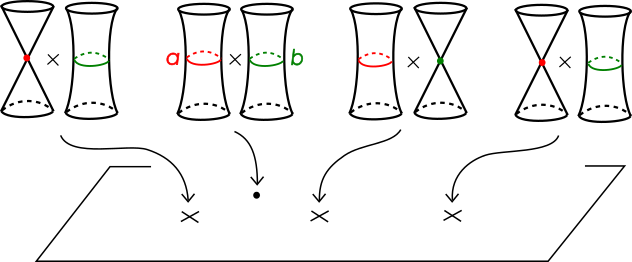
\includegraphics[width=0.7\linewidth]{MLB-for-W_0}
 \caption{Morse--Bott--Lefschetz fibration on $(W_0, \omega_0)$. The crosses in the base denote singular values, and the dot a regular one.
 \label{fig:MLB-for-W_0}}
\end{figure}

\begin{rmk}\label{rmk:classify 3-spheres}
 The analysis from \cite{Smith-Wemyss} did not yield a classification of Lagrangian 3-spheres in~$W_0$, in contrast to the case for the closely related double bubble plumbing from Section~\ref{sec:double-bubble} (called~$W_1$ in op.~cit.). The space~$W_0$ is an affine quartic, and the total space of a conic fibration over~$T^*S^2$, which in turn is a conic fibration over a plane. Note that~$W_0$ admits a $\bC^*$-action, and any Lagrangian sphere defines an equivariant module, cf.~\cite[Proposition~6.5]{Auroux-Smith} which follows \cite[Corollary~A.12]{Seidel-dilating}. Recent speculations of Lekili and Segal~\cite{LS} give a description of the $(\bC^*)^2$-equivariant Fukaya category of~$W_0$, for the fibrewise action, in terms of a partially wrapped Fukaya category of a thrice-punctured plane. Starting from this, and using classification results for objects in Fukaya categories of surfaces, one could hope to classify Lagrangian 3-spheres in~$W_0$. This would be a rather different route to classification than that taken for $W_1$ in \cite{Hara-Wemyss, Smith-Wemyss}, closer to the recent arguments of~\cite{Xie-Li} (cf.~Remark~\ref{rmk:multibubble as surface category} above).
\end{rmk}

One easily checks that $H^2(W_0;\bZ) \cong \bZ$, so there is an inexact deformation $\omega_t$ of the symplectic form $\omega_0$ on $W_0$. In fact, this can be realised geometrically. Note that the original Morse--Bott--Lefschetz fibration on $W_0$ has monodromies on $\bC^*\times \bC^*$ which are given by
\[
\tau_a \times \{{\rm id}\}, \quad \{{\rm id}\} \times \tau_b, \quad \tau_a \times \{{\rm id}\},
\]
respectively, where $\tau_{\bullet}$ denotes the Dehn twist in the curve $\bullet$. The corresponding vanishing cycles, for appropriate vanishing paths, are $\{a,b,a\}$ in a hopefully obvious shorthand. Let $\phi_x$ denote the symplectomorphism of $\bC^* = \bR\times S^1$ which is given by a translation by $x$ in the $\bR$-factor, i.e.,~the symplectomorphism (unique up to Hamiltonian isotopy) with flux $x \in H^1(\bC^*;\bR)\cong \bR$.

\begin{lem}
The space $(W_0,\omega_t)$ admits a Morse--Bott--Lefschetz fibration with the same monodromies as before, but the vanishing cycles associated to the previously chosen vanishing paths are now $\{a,b,(\phi_t\times \id)(a)\}$.
\end{lem}

\begin{proof}
 Cut $W_0$ along the codimension one hypersurface which is the preimage of a vertical line in $\bC$ disjoint from the critical values of the MBL fibration, and such that the two critical values with vanishing cycle $a$ lie on either side of the cut; and reglue by the map given by translation on the first factor of the fibre and the identity on the second. This is a symplectomorphism, so the result is again a symplectic manifold, manifestly diffeomorphic to $W_0$ (we have only changed the locally Hamiltonian structure of the fibration; the re-gluing is by a map smoothly isotopic to the identity). Since the change in symplectic structure is localised away from the critical submanifolds, the local monodromies are unchanged, but at least one of the vanishing paths will cross the cut locus and the corresponding vanishing cycle will therefore change as indicated.
\end{proof}

\begin{cor}\label{cor:disjoinable}
 Let $0 \neq t \in \bR$. In the inexact deformation $(W_0,\omega_t)$, the two core Lagrangian $3$-spheres are disjoint.
\end{cor}

\begin{proof}
 The two matching spheres now meet the central singular fibre in copies of a circle $S^1 \times \{pt\} \subset \bC^*\times (\bC\vee\bC)$, where the (first factor) circles for the two different matching spheres differ by a translation of flux $t$.
\end{proof}

Note that the Lagrangian $S^1 \times S^2 \subset (W_0,\omega_0)$ which was fibred over a matching path between the outermost critical values is no longer Lagrangian, since the two-sphere factor has acquired positive area. The space $W_0$ carries an action by symplectic parallel transport of the mixed braid group $M{\rm Br}_3$. Consider the generator given by the lift of a half-twist, in $\bC$, along a matching path between the two critical values of type $a$. Observe that this is also naturally a lift under a~map $W_0 \to T^*S^2$ (forgetting the second coordinate on each fibre) of the Dehn twist in the $S^2$, which no longer has infinite order after the inexact deformation of $\omega$. Similarly, the twists in the core spheres now commute, since these are now disjoint.

The conifold mirror $X$ introduced in \eqref{eqn:conifold mirror} has $H^2(X;\bR) \cong \bR^2_{s,t}$. Let $(X, \omega_{s,t})$ be a corresponding inexact deformation of the Weinstein manifold $X$. We obtain a geometric model for $(X,\omega_{s,t})$ by considering the Morse--Bott--Lefschetz fibration over $\bC^*$ with two singular fibres with monodromies
\[
\tau_a \times \id, \ \{\phi_s\} \times \{\phi_t\} \ \mathrm{and} \ \id \times \tau_b
\]
around $-1$, $0$ and $ 1$, respectively, for the obvious three loops based at $i \in \bC^\ast$.
Note that, as one iterates monodromies around the critical fibres, the fluxes add, so one finds the following.

\begin{cor}
 Let $s$, $t$ both be non-zero. The deformation $(X,\omega_{s,t})$ of the conifold mirror contains infinitely many pairwise disjoint Lagrangian 3-spheres.
\end{cor}

\begin{proof}
 Consider matching paths between the two critical values with larger and larger winding number around the origin; given two distinct such, at any intersection point of the base matching paths, the winding number difference means at least one of the fibrewise factors has been translated by a non-trivial flux. See Figure~\ref{fig:Inexact-conifold-with-spheres}.
\end{proof}

\begin{figure}
 \centering
 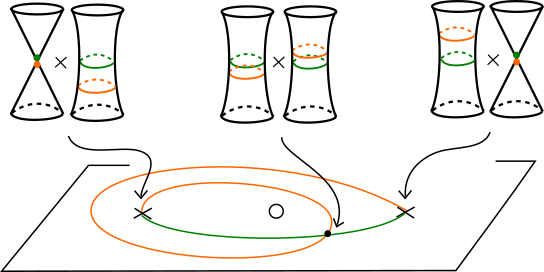
\includegraphics[width=0.7\linewidth]{Inexact-conifold-with-spheres}
 \caption{Example of disjoint Lagrangian matching spheres in $(X, \omega_{s,t})$.}
 \label{fig:Inexact-conifold-with-spheres}
\end{figure}

\begin{rmk}
 The Lagrangian spheres associated to matching paths are still the only Lagrangian spheres we can `see' after deformation, but we no longer have even a tentative route to a~classification guaranteeing that these are the only spherical objects.
\end{rmk}


Each Lagrangian matching sphere has an associated Dehn twist. Disjointness implies these twists now commute. By considering the action on the set of graded Lagrangian spheres, and using that $\tau_L(L)=L[-1]$ but $\tau_L$ does not shift $K$ if $K \cap L = \emptyset$, one sees that the homomorphism from $\bZ^{\oplus \infty} \to \pi_0\Symp_c^{\rm gr}(X,\omega_{s,t})$ will be injective when $s,t \neq 0$.
\begin{qn}
 Does the resulting homomorphism $\bZ^{\oplus \infty} \to \pi_0\Symp_c(X,\omega_{s,t})$ split?
\end{qn}

\begin{rmk}
 The approach suggested in Remark \ref{rmk:classify 3-spheres} does not obviously survive the deformation of the symplectic form, since this has no obvious interpretation in the model for the equivariant category formulated on the reduced space of the $\bC^*$-actions.
\end{rmk}


 As a digression, we note that one can `compactify' the preceding example:


 \begin{prop}
 There is a compact symplectic six-manifold which contains infinitely many pairwise disjoint Lagrangian $3$-spheres.
 \end{prop}


\begin{proof}
 We consider a Morse--Bott--Lefschetz (MBL) fibration with fibre $T^2\times T^2$ constructed as follows. Begin with the four-manifold which is a symplectic $T^2$-fibration over a torus with monodromies $\id$ and $\phi_s$ for some flux $s$. This is locally Hamiltonian, so admits a symplectic structure. We fibre sum this with a rational elliptic surface, to obtain a symplectic fibration $Z \to T^2$ over the two-torus with a dozen nodal singular fibres lying over a disc $D \subset T^2$, still with monodromies $\{id,\phi_s\}$.

 We now take two copies $Z$ and $Z'$ of this four-manifold, where $Z$ has monodromies $\{\id,\phi_s\}$ and $Z'$ has monodromies $\{\phi_t,\id\}$ (so the flux has switched to the other factor of the base). We also insist that the singular fibres for $Z$ (resp.~$Z'$) lie over disjoint discs $D,D' \subset T^2$. Now take the fibre product $Z \times_{T^2} Z'$. The disjointness of $D$ and $D'$ means that at most one of the two input fibrations has a singular point over a given $p\in T^2$, which ensures that the fibre product is the total space of a MBL fibration with general fibre~$T^4$.

 We now impose the condition that the non-trivial fluxes $s,t \in H^1(T^2;\bR) \cong \bR^2$ are irrational, so have infinite order in the symplectomorphism group of the fibre. One can construct Lagrangian matching spheres in the total space exactly as in the inexact conifold. The irrationality of the fluxes ensures that the spheres associated to matching paths which meet in the base, as in Figure~\ref{fig:Inexact-conifold-with-spheres}, are still disjoint in the total space. This is because the iterated translations of a compact two-torus in $T^4$ by an irrational angle in a complementary direction (i.e., writing $T^4 = T^2 \times T^2$ and translating the first factor by iterations of an irrational flux in the second factor) remain pairwise disjoint for all iterations.
\end{proof}

Such examples do not seem to have been observed previously.


\begin{thebibliography}{99}
\footnotesize\itemsep=0pt

\bibitem{Abouzaid-Seidel:Viterbo}
Abouzaid M., Seidel P., An open string analogue of {V}iterbo functoriality,
 \href{https://doi.org/10.2140/gt.2010.14.627}{\textit{Geom. Topol.}}
 \textbf{14} (2010), 627--718,
 \href{http://arxiv.org/abs/0712.3177}{arXiv:0712.3177}.

\bibitem{AbSm-plumbing}
Abouzaid M., Smith I., Exact {L}agrangians in plumbings,
 \href{https://doi.org/10.1007/s00039-012-0162-y}{\textit{Geom. Funct. Anal.}}
 \textbf{22} (2012), 785--831,
 \href{http://arxiv.org/abs/1107.0129}{arXiv:1107.0129}.

\bibitem{Akaho-Joyce}
Akaho M., Joyce D., Immersed {L}agrangian {F}loer theory,
 \href{https://doi.org/10.4310/jdg/1303219427}{\textit{J.~Differential Geom.}}
 \textbf{86} (2010), 381--500,
 \href{http://arxiv.org/abs/0803.0717}{arXiv:0803.0717}.

\bibitem{Amiot}
Amiot C., Cluster categories for algebras of global dimension 2 and quivers
 with potential, \href{https://doi.org/10.5802/aif.2499}{\textit{Ann. Inst.
 Fourier (Grenoble)}} \textbf{59} (2009), 2525--2590,
 \href{http://arxiv.org/abs/0805.1035}{arXiv:0805.1035}.

\bibitem{August-Wemyss}
August J., Wemyss M., Stability conditions for contraction algebras,
 \href{https://doi.org/10.1017/fms.2022.65}{\textit{Forum Math. Sigma}}
 \textbf{10} (2022), e73, 20~pages,
 \href{http://arxiv.org/abs/1907.12756}{arXiv:1907.12756}.

\bibitem{Auroux-Smith}
Auroux D., Smith I., Fukaya categories of surfaces, spherical objects and
 mapping class groups,
 \href{https://doi.org/10.1017/fms.2021.21}{\textit{Forum Math. Sigma}}
 \textbf{9} (2021), e26, 50~pages,
 \href{http://arxiv.org/abs/2006.09689}{arXiv:2006.09689}.

\bibitem{BJK}
Bae H., Jeong W., Kim J., Cluster categories from {F}ukaya categories,
 \href{https://doi.org/10.1142/S0129167X25500193}{\textit{Internat.~J. Math.}}
 \textbf{36} (2025), 2550019, 30~pages,
 \href{http://arxiv.org/abs/2209.09442}{arXiv:2209.09442}.

\bibitem{Baur-Marsh}
Baur K., Marsh R.J., A geometric description of {$m$}-cluster categories,
 \href{https://doi.org/10.1090/S0002-9947-08-04441-3}{\textit{Trans. Amer.
 Math. Soc.}} \textbf{360} (2008), 5789--5803,
 \href{http://arxiv.org/abs/math.RA/0607151}{arXiv:math.RA/0607151}.

\bibitem{Birman-Hilden}
Birman J.S., Hilden H.M., On isotopies of homeomorphisms of {R}iemann surfaces,
 \href{https://doi.org/10.2307/1970830}{\textit{Ann. of Math.}} \textbf{97}
 (1973), 424--439.

\bibitem{Blanc}
Blanc J., Symplectic birational transformations of the plane,
 \href{https://doi.org/10.18910/25084}{\textit{Osaka~J. Math.}} \textbf{50}
 (2013), 573--590, \href{http://arxiv.org/abs/1012.0706}{arXiv:1012.0706}.

\bibitem{BEE}
Bourgeois F., Ekholm T., Eliashberg Y., Effect of {L}egendrian surgery (with an
 appendix by {S}heel {G}anatra and {M}aksim {M}aydanskiy),
 \href{https://doi.org/10.2140/gt.2012.16.301}{\textit{Geom. Topol.}}
 \textbf{16} (2012), 301--389,
 \href{http://arxiv.org/abs/0911.0026}{arXiv:0911.0026}.

\bibitem{BS}
Bridgeland T., Smith I., Quadratic differentials as stability conditions,
 \href{https://doi.org/10.1007/s10240-014-0066-5}{\textit{Publ. Math. Inst.
 Hautes \'{E}tudes Sci.}} \textbf{121} (2015), 155--278,
 \href{http://arxiv.org/abs/1302.7030}{arXiv:1302.7030}.

\bibitem{Brustle-YuQiu}
Br\"{u}stle T., Qiu Y., Tagged mapping class groups: {A}uslander--{R}eiten
 translation,
 \href{https://doi.org/10.1007/s00209-015-1405-z}{\textit{Math.~Z.}}
 \textbf{279} (2015), 1103--1120,
 \href{http://arxiv.org/abs/1212.0007}{arXiv:1212.0007}.

\bibitem{Brustle-Zhang}
Br\"{u}stle T., Zhang J., On the cluster category of a marked surface without
 punctures, \href{https://doi.org/10.2140/ant.2011.5.529}{\textit{Algebra
 Number Theory}} \textbf{5} (2011), 529--566,
 \href{http://arxiv.org/abs/1005.2422}{arXiv:1005.2422}.

\bibitem{BRT}
Buan A.B., Reiten I., Thomas H., From {$m$}-clusters to {$m$}-noncrossing
 partitions via exceptional sequences,
 \href{https://doi.org/10.1007/s00209-011-0906-7}{\textit{Math.~Z.}}
 \textbf{271} (2012), 1117--1139,
 \href{http://arxiv.org/abs/1007.0928}{arXiv:1007.0928}.

\bibitem{CPU}
Chan K., Pomerleano D., Ueda K., Lagrangian torus fibrations and homological
 mirror symmetry for the conifold,
 \href{https://doi.org/10.1007/s00220-015-2477-7}{\textit{Comm. Math. Phys.}}
 \textbf{341} (2016), 135--178,
 \href{http://arxiv.org/abs/1305.0968}{arXiv:1305.0968}.

\bibitem{Christ}
Christ M., Ginzburg algebras of triangulated surfaces and perverse schobers,
 \href{https://doi.org/10.1017/fms.2022.1}{\textit{Forum Math. Sigma}}
 \textbf{10} (2022), e8, 72~pages,
 \href{http://arxiv.org/abs/2101.01939}{arXiv:2101.01939}.

\bibitem{DRE}
Dimitroglou~Rizell G., Evans J.D., Exotic spheres and the topology of
 symplectomorphism groups,
 \href{https://doi.org/10.1112/jtopol/jtv007}{\textit{J.~Topol.}} \textbf{8}
 (2015), 586--602, \href{http://arxiv.org/abs/1407.3173}{arXiv:1407.3173}.

\bibitem{Disarlo}
Disarlo V., Combinatorial rigidity of arc complexes,
 \href{http://arxiv.org/abs/1505.08080}{arXiv:1505.08080}.

\bibitem{Dolgachev-book}
Dolgachev I.V., Classical algebraic geometry. {A}~modern view,
 \href{https://doi.org/10.1017/CBO9781139084437}{Cambridge University Press},
 Cambridge, 2012.

\bibitem{Donovan-Wemyss}
Donovan W., Wemyss M., Twists and braids for general 3-fold flops,
 \href{https://doi.org/10.4171/JEMS/868}{\textit{J.~Eur. Math. Soc. (JEMS)}}
 \textbf{21} (2019), 1641--1701,
 \href{http://arxiv.org/abs/1504.05320}{arXiv:1504.05320}.

\bibitem{Drinfeld}
Drinfeld V., D{G} quotients of {DG} categories,
 \href{https://doi.org/10.1016/j.jalgebra.2003.05.001}{\textit{J.~Algebra}}
 \textbf{272} (2004), 643--691,
 \href{http://arxiv.org/abs/math.KT/0210114}{arXiv:math.KT/0210114}.

\bibitem{Evans}
Evans J.D., Symplectic mapping class groups of some {S}tein and rational
 surfaces,
 \href{https://doi.org/10.4310/jsg.2011.v9.n1.a4}{\textit{J.~Symplectic
 Geom.}} \textbf{9} (2011), 45--82,
 \href{http://arxiv.org/abs/0909.5622}{arXiv:0909.5622}.

\bibitem{Fan-Lai}
Fan Y.-W., Lai K.-W., Mirror symmetry for lattice-polarised abelian surfaces,
 \href{http://arxiv.org/abs/2602.04232}{arXiv:2602.04232}.

\bibitem{FST}
Fomin S., Shapiro M., Thurston D., Cluster algebras and triangulated surfaces.
 {I}. {C}luster complexes,
 \href{https://doi.org/10.1007/s11511-008-0030-7}{\textit{Acta Math.}}
 \textbf{201} (2008), 83--146,
 \href{http://arxiv.org/abs/math.RA/0608367}{arXiv:math.RA/0608367}.

\bibitem{GGV}
Ganatra S., Gao Y., Venkatesh S., Rabinowitz {F}ukaya categories and the
 categorical formal punctured neighborhood of infinity,
 \href{http://arxiv.org/abs/2212.14863}{arXiv:2212.14863}.

\bibitem{GPS}
Ganatra S., Pardon J., Shende V., Covariantly functorial wrapped {F}loer theory
 on {L}iouville sectors,
 \href{https://doi.org/10.1007/s10240-019-00112-x}{\textit{Publ. Math. Inst.
 Hautes \'{E}tudes Sci.}} \textbf{131} (2020), 73--200,
 \href{http://arxiv.org/abs/1706.03152}{arXiv:1706.03152}.

\bibitem{Ginzburg}
Ginzbug V., Calabi--{Y}au algebras,
 \href{http://arxiv.org/abs/math.SG/0612139}{arXiv:math.SG/0612139}.

\bibitem{Groman}
Groman Y., Floer theory and reduced cohomology on open manifolds,
 \href{https://doi.org/10.2140/gt.2023.27.1273}{\textit{Geom. Topol.}}
 \textbf{27} (2023), 1273--1390,
 \href{http://arxiv.org/abs/1510.04265}{arXiv:1510.04265}.

\bibitem{Gromov-1985}
Gromov M., Pseudo holomorphic curves in symplectic manifolds,
 \href{https://doi.org/10.1007/BF01388806}{\textit{Invent. Math.}} \textbf{82}
 (1985), 307--347.

\bibitem{GHK2}
Gross M., Hacking P., Keel S., Moduli of surfaces with an anti-canonical cycle,
 \href{https://doi.org/10.1112/S0010437X14007611}{\textit{Compos. Math.}}
 \textbf{151} (2015), 265--291,
 \href{http://arxiv.org/abs/1211.6367}{arXiv:1211.6367}.

\bibitem{Hacking-Keating-1}
Hacking P., Keating A., Homological mirror symmetry for log {C}alabi--{Y}au
 surfaces (with an appendix by {W}endelin {L}utz),
 \href{https://doi.org/10.2140/gt.2022.26.3747}{\textit{Geom. Topol.}}
 \textbf{26} (2022), 3747--3833,
 \href{http://arxiv.org/abs/2005.05010}{arXiv:2005.05010}.

\bibitem{Hacking-Keating-2}
Hacking P., Keating A., Symplectomorphisms of some {W}einstein 4-manifolds,
 \href{https://doi.org/10.2140/gt.2026.30.645}{\textit{Geom. Topol.}}
 \textbf{30} (2026), 645--699,
 \href{http://arxiv.org/abs/2112.06797}{arXiv:2112.06797}.

\bibitem{Hacking-Keating-3}
Hacking P., Keating A., Homological mirror symmetry for projective {K}3,
 \href{http://arxiv.org/abs/2503.05680}{arXiv:2503.05680}.

\bibitem{Hara-Wemyss}
Hara W., Wemyss M., Spherical objects in dimensions two and three,
 \href{https://doi.org/10.4171/jems/1504}{\textit{J.~Eur. Math. Soc. (JEMS)}}
 \textbf{28} (2026), 1771--1808,
 \href{http://arxiv.org/abs/2205.11552}{arXiv:2205.11552}.

\bibitem{Hirano-Wemyss}
Hirano Y., Wemyss M., Stability conditions for 3-fold flops,
 \href{https://doi.org/10.1215/00127094-2022-0097}{\textit{Duke Math.~J.}}
 \textbf{172} (2023), 3105--3173,
 \href{http://arxiv.org/abs/1907.09742}{arXiv:1907.09742}.

\bibitem{Hu-Krah}
Hu X., Krah J., Autoequivalences of blow-ups of minimal surfaces,
 \href{https://doi.org/10.1112/blms.13131}{\textit{Bull. Lond. Math. Soc.}}
 \textbf{56} (2024), 3257--3267,
 \href{http://arxiv.org/abs/2310.17938}{arXiv:2310.17938}.

\bibitem{Ikeda}
Ikeda A., Stability conditions on {${\rm CY}_N$} categories associated to
 {$A_n$}-quivers and period maps,
 \href{https://doi.org/10.1007/s00208-016-1375-4}{\textit{Math. Ann.}}
 \textbf{367} (2017), 1--49,
 \href{http://arxiv.org/abs/1405.5492}{arXiv:1405.5492}.

\bibitem{Ionescu}
Ionescu P., Deformations of complete intersections, \textit{Rev. Roumaine Math.
 Pures Appl.} \textbf{25} (1980), 751--758.

\bibitem{Jacquet-Malo}
Jacquet-Malo L., A bijection between {$m$}-cluster-tilting objects and
 {$(m+2)$}-angulations in {$m$}-cluster categories,
 \href{https://doi.org/10.1016/j.jalgebra.2021.11.041}{\textit{J.~Algebra}}
 \textbf{595} (2022), 581--632,
 \href{http://arxiv.org/abs/1706.06866}{arXiv:1706.06866}.

\bibitem{Jannaud}
Jannaud A., Dehn--{S}eidel twist, ${C}^0$ symplectic topology and barcodes,
 \href{http://arxiv.org/abs/2101.07878}{arXiv:2101.07878}.

\bibitem{Kalck-Yang}
Kalck M., Yang D., Relative singularity categories {I}: {A}uslander
 resolutions, \href{https://doi.org/10.1016/j.aim.2016.06.011}{\textit{Adv.
 Math.}} \textbf{301} (2016), 973--1021,
 \href{http://arxiv.org/abs/1205.1008}{arXiv:1205.1008}.

\bibitem{Karabas-Lee}
Karabas D., Lee S., The wrapped {F}ukaya category of plumbings,
 \href{https://doi.org/10.4310/jsg.250820172316}{\textit{J.~Symplectic Geom.}}
 \textbf{23} (2025), 853--949,
 \href{http://arxiv.org/abs/2405.10783}{arXiv:2405.10783}.

\bibitem{Kartal:algebraic}
Kartal Y.B., Algebraic sheaves of {F}loer homology groups via algebraic torus
 actions on the {F}ukaya category,
 \href{http://arxiv.org/abs/2109.12256}{arXiv:2109.12256}.

\bibitem{Keating-Smith}
Keating A., Smith I., Symplectomorphisms and spherical objects in the conifold
 smoothing, \href{https://doi.org/10.1112/S0010437X24007425}{\textit{Compos.
 Math.}} \textbf{160} (2024), 2738--2773,
 \href{http://arxiv.org/abs/2301.10525}{arXiv:2301.10525}.

\bibitem{KS:corr}
Keating A., Smith I., Corrigendum to ``Symplectomorphisms and spherical objects
 in the conifold smoothing'',
 \href{https://doi.org/10.1017/S0010437X26103297}{\textit{Compos. Math.}}
 \textbf{162} (2026), 1046--1051.

\bibitem{Keating-Ward}
Keating A., Ward A., A universal mirror to $\bigl(\mathbb{P}^2,\Omega\bigr)$ as
 a~birational object,
 \href{http://arxiv.org/abs/2408.03764}{arXiv:2408.03764}.

\bibitem{Keller-Yang}
Keller B., Yang D., Derived equivalences from mutations of quivers with
 potential, \href{https://doi.org/10.1016/j.aim.2010.09.019}{\textit{Adv.
 Math.}} \textbf{226} (2011), 2118--2168,
 \href{http://arxiv.org/abs/0906.0761}{arXiv:0906.0761}.

\bibitem{Khovanov-Seidel}
Khovanov M., Seidel P., Quivers, {F}loer cohomology, and braid group actions,
 \href{https://doi.org/10.1090/S0894-0347-01-00374-5}{\textit{J.~Amer. Math.
 Soc.}} \textbf{15} (2002), 203--271,
 \href{http://arxiv.org/abs/math.QA/0006056}{arXiv:math.QA/0006056}.

\bibitem{King-QiuYu-cluster}
King A., Qiu Y., Exchange graphs and {E}xt quivers,
 \href{https://doi.org/10.1016/j.aim.2015.08.017}{\textit{Adv. Math.}}
 \textbf{285} (2015), 1106--1154,
 \href{http://arxiv.org/abs/1109.2924}{arXiv:1109.2924}.

\bibitem{King-QiuYu}
King A., Qiu Y., Cluster exchange groupoids and framed quadratic differentials,
 \href{https://doi.org/10.1007/s00222-019-00932-y}{\textit{Invent. Math.}}
 \textbf{220} (2020), 479--523,
 \href{http://arxiv.org/abs/1805.00030}{arXiv:1805.00030}.

\bibitem{Lalonde-Pinsonnault}
Lalonde F., Pinsonnault M., The topology of the space of symplectic balls in
 rational 4-manifolds,
 \href{https://doi.org/10.1215/S0012-7094-04-12223-7}{\textit{Duke Math.~J.}}
 \textbf{122} (2004), 347--397,
 \href{http://arxiv.org/abs/math.SG/0207096}{arXiv:math.SG/0207096}.

\bibitem{LS}
Lekili Y., Segal E., Equivariant {F}ukaya categories at singular values,
 \href{https://doi.org/10.1017/s0017089525100487}{\textit{Glasg. Math.~J.}}
 \textbf{68} (2026), 197--221,
 \href{http://arxiv.org/abs/2304.10969}{arXiv:2304.10969}.

\bibitem{Lekili-Ueda}
Lekili Y., Ueda K., Homological mirror symmetry for {M}ilnor fibers via moduli
 of {$A_\infty$}-structures,
 \href{https://doi.org/10.1112/topo.12248}{\textit{J.~Topol.}} \textbf{15}
 (2022), 1058--1106, \href{http://arxiv.org/abs/1806.04345}{arXiv:1806.04345}.

\bibitem{Li-Li-Wu-1}
Li J., Li T.-J., Wu W., The symplectic mapping class group of {$\mathbb
 CP^2\#n\overline{\mathbb CP^2}$} with {$n \le 4$},
 \href{https://doi.org/10.1307/mmj/1434731926}{\textit{Michigan Math.~J.}}
 \textbf{64} (2015), 319--333,
 \href{http://arxiv.org/abs/1310.7329}{arXiv:1310.7329}.

\bibitem{Li-Li-Wu-2}
Li J., Li T.-J., Wu W., Symplectic {$(-2)$}-spheres and the symplectomorphism
 group of small rational 4-manifolds~{II},
 \href{https://doi.org/10.1090/tran/8517}{\textit{Trans. Amer. Math. Soc.}}
 \textbf{375} (2022), 1357--1410,
 \href{http://arxiv.org/abs/1911.11073}{arXiv:1911.11073}.

\bibitem{Li-Li-Wu}
Li J., Li T.-J., Wu W., Symplectic {T}orelli groups of rational surfaces,
 \href{http://arxiv.org/abs/2212.01873}{arXiv:2212.01873}.

\bibitem{Li-Wu}
Li T.-J., Wu W., Lagrangian spheres, symplectic surfaces and the symplectic
 mapping class group,
 \href{https://doi.org/10.2140/gt.2012.16.1121}{\textit{Geom. Topol.}}
 \textbf{16} (2012), 1121--1169,
 \href{http://arxiv.org/abs/1012.4146}{arXiv:1012.4146}.

\bibitem{Looijenga}
Looijenga E., Artin groups and the fundamental groups of some moduli spaces,
 \href{https://doi.org/10.1112/jtopol/jtm009}{\textit{J.~Topol.}} \textbf{1}
 (2008), 187--216,
 \href{http://arxiv.org/abs/math.AG/9801117}{arXiv:math.AG/9801117}.

\bibitem{Lunts-Orlov}
Lunts V.A., Orlov D.O., Uniqueness of enhancement for triangulated categories,
 \href{https://doi.org/10.1090/S0894-0347-10-00664-8}{\textit{J.~Amer. Math.
 Soc.}} \textbf{23} (2010), 853--908,
 \href{http://arxiv.org/abs/0908.4187}{arXiv:0908.4187}.

\bibitem{Margalit-Winarski}
Margalit D., Winarski R.R., Braid groups and mapping class groups: {T}he
 {B}irman--{H}ilden theory,
 \href{https://doi.org/10.1112/blms.12456}{\textit{Bull. Lond. Math. Soc.}}
 \textbf{53} (2021), 643--659.

\bibitem{Munoz-Echaniz}
Mu\~noz Ech\'aniz J., Configurations of {L}agrangian spheres in {$K3$}
 surfaces, \href{http://arxiv.org/abs/2507.15039}{arXiv:2507.15039}.

\bibitem{Okada-Spotti-Sun}
Odaka Y., Spotti C., Sun S., Compact moduli spaces of {D}el {P}ezzo surfaces
 and {K}\"{a}hler--{E}instein metrics,
 \href{https://doi.org/10.4310/jdg/1452002879}{\textit{J.~Differential Geom.}}
 \textbf{102} (2016), 127--172,
 \href{http://arxiv.org/abs/1210.0858}{arXiv:1210.0858}.

\bibitem{Pinsonnault}
Pinsonnault M., Symplectomorphism groups and embeddings of balls into rational
 ruled 4-manifolds,
 \href{https://doi.org/10.1112/S0010437X0700334X}{\textit{Compos. Math.}}
 \textbf{144} (2008), 787--810,
 \href{http://arxiv.org/abs/math.SG/0603310}{arXiv:math.SG/0603310}.

\bibitem{Pomerleano}
Pomerleano D., Intrinsic mirror symmetry and categorical crepant resolutions,
 \href{http://arxiv.org/abs/2103.01200}{arXiv:2103.01200}.

\bibitem{QiuYu:spherical-twist-group}
Qiu Y., Decorated marked surfaces: spherical twists versus braid twists,
 \href{https://doi.org/10.1007/s00208-015-1339-0}{\textit{Math. Ann.}}
 \textbf{365} (2016), 595--633,
 \href{http://arxiv.org/abs/1407.0806}{arXiv:1407.0806}.

\bibitem{Qiu-Woolf}
Qiu Y., Woolf J., Contractible stability spaces and faithful braid group
 actions, \href{https://doi.org/10.2140/gt.2018.22.3701}{\textit{Geom.
 Topol.}} \textbf{22} (2018), 3701--3760,
 \href{http://arxiv.org/abs/1407.5986}{arXiv:1407.5986}.

\bibitem{Reid}
Reid M., The complete intersection of two or more quadrics, {U}niversity of
 Cambridge, 1972, available at
 \url{https://mreid.warwick.ac.uk/3folds/qu.pdf}.

\bibitem{JieRen}
Ren J., Calabi--{Y}au categories and graded quivers with potential,
 \href{http://arxiv.org/abs/2402.03330}{arXiv:2402.03330}.

\bibitem{Ritter}
Ritter A.F., Topological quantum field theory structure on symplectic
 cohomology, \href{https://doi.org/10.1112/jtopol/jts038}{\textit{J.~Topol.}}
 \textbf{6} (2013), 391--489,
 \href{http://arxiv.org/abs/1003.1781}{arXiv:1003.1781}.

\bibitem{Salter}
Salter N., On the monodromy group of the family of smooth quintic plane curves,
 \href{https://doi.org/10.1017/S0017089524000284}{\textit{Glasg. Math.~J.}}
 \textbf{67} (2025), 163--184,
 \href{http://arxiv.org/abs/1610.04920}{arXiv:1610.04920}.

\bibitem{Schmutz}
Schmutz~Schaller P., Mapping class groups of hyperbolic surfaces and
 automorphism groups of graphs,
 \href{https://doi.org/10.1023/A:1002672721132}{\textit{Compositio Math.}}
 \textbf{122} (2000), 243--260.

\bibitem{Seidel_T*S2_unpublished}
Seidel P., Symplectic automorphisms of ${T}^*{S}^2$,
 \href{http://arxiv.org/abs/math.DG/9803084}{arXiv:math.DG/9803084}.


\bibitem{Seidel:graded}
Seidel P., Graded {L}agrangian submanifolds,
 \href{https://doi.org/10.24033/bsmf.2365}{\textit{Bull. Soc. Math. France}}
 \textbf{128} (2000), 103--149.

\bibitem{Seidel:bias}
Seidel P., A~biased view of symplectic cohomology, in Current Developments in
 Mathematics,
 \href{https://doi.org/10.4310/CDM.2006.v2006.n1.a4}{International Press},
 Somerville, MA, 2008, 211--253,
 \href{http://arxiv.org/abs/0704.2055}{arXiv:0704.2055}.

\bibitem{Seidel:FCPLT}
Seidel P., Fukaya categories and {P}icard--{L}efschetz theory, \textit{Zur. Lect. Adv.
 Math.}, \href{https://doi.org/10.4171/063}{European Mathematical Society},
 Z\"urich, 2008.

\bibitem{Seidel_lectures_4Dtwists}
Seidel P., Lectures on four-dimensional {D}ehn twists, in Symplectic
 4-Manifolds and Algebraic Surfaces, \textit{Lecture Notes in Math.}, Vol.~1938, \href{https://doi.org/10.1007/978-3-540-78279-7_4}{Springer}, Berlin,
 2008, 231--267,
 \href{http://arxiv.org/abs/math.SG/0309012}{arXiv:math.SG/0309012}.

\bibitem{Seidel:Flux}
Seidel P., Abstract analogues of flux as symplectic invariants,
 \href{https://doi.org/10.24033/msmf.447}{\textit{M\'em. Soc. Math. Fr.
 (N.S.)}} (2014), 135,
 \href{http://arxiv.org/abs/1108.0394}{arXiv:1108.0394}.

\bibitem{Seidel:categorical_dynamics}
Seidel P., Lectures on categorical dynamics and symplectic topology,
 {U}npublished manuscript, 2014, available at
 \url{http://math.mit.edu/~seidel/}.

\bibitem{Seidel-dilating}
Seidel P., Picard--{L}efschetz theory and dilating {$\mathbb{C}^*$}-actions,
 \href{https://doi.org/10.1112/jtopol/jtv029}{\textit{J.~Topol.}} \textbf{8}
 (2015), 1167--1201, \href{http://arxiv.org/abs/1403.7571}{arXiv:1403.7571}.

\bibitem{Sheridan-Smith:K3}
Sheridan N., Smith I., Symplectic topology of {$K3$} surfaces via mirror
 symmetry, \href{https://doi.org/10.1090/jams/946}{\textit{J.~Amer. Math.
 Soc.}} \textbf{33} (2020), 875--915,
 \href{http://arxiv.org/abs/1709.09439}{arXiv:1709.09439}.

\bibitem{Smith}
Smith I., Floer cohomology and pencils of quadrics,
 \href{https://doi.org/10.1007/s00222-011-0364-1}{\textit{Invent. Math.}}
 \textbf{189} (2012), 149--250,
 \href{http://arxiv.org/abs/1006.1099}{arXiv:1006.1099}.

\bibitem{Smith:quiver}
Smith I., Quiver algebras as {F}ukaya categories,
 \href{https://doi.org/10.2140/gt.2015.19.2557}{\textit{Geom. Topol.}}
 \textbf{19} (2015), 2557--2617,
 \href{http://arxiv.org/abs/1309.0452}{arXiv:1309.0452}.

\bibitem{Smith-Wemyss}
Smith I., Wemyss M., Double bubble plumbings and two-curve flops,
 \href{https://doi.org/10.1007/s00029-023-00828-z}{\textit{Selecta
 Math.~(N.S.)}} \textbf{29} (2023), 29, 62~pages,
 \href{http://arxiv.org/abs/2010.10114}{arXiv:2010.10114}.

\bibitem{Song-Tillmann}
Song Y., Tillmann U., Braids, mapping class groups, and categorical delooping,
 \href{https://doi.org/10.1007/s00208-007-0117-z}{\textit{Math. Ann.}}
 \textbf{339} (2007), 377--393, \href{http://arxiv.org/abs/math.AT/0609597}{arXiv:math.AT/0609597}.

\bibitem{TV}
To\"{e}n B., Vaqui\'e M., Moduli of objects in dg-categories,
 \href{https://doi.org/10.1016/j.ansens.2007.05.001}{\textit{Ann. Sci.
 \'{E}cole Norm. Sup. (4)}} \textbf{40} (2007), 387--444, \href{http://arxiv.org/abs/math.AG/0503269}{arXiv:math.AG/0503269}.

\bibitem{Uehara}
Uehara H., A trichotomy for the autoequivalence groups on smooth projective
 surfaces, \href{https://doi.org/10.1090/tran/7439}{\textit{Trans. Amer. Math.
 Soc.}} \textbf{371} (2019), 3529--3547, \href{http://arxiv.org/abs/1704.00292}{arXiv:1704.00292}.

\bibitem{Wendl}
Wendl C., Strongly fillable contact manifolds and {$J$}-holomorphic foliations,
 \href{https://doi.org/10.1215/00127094-2010-001}{\textit{Duke Math.~J.}}
 \textbf{151} (2010), 337--384, \href{http://arxiv.org/abs/0806.3193}{arXiv:0806.3193}.

\bibitem{Wu}
Wu W., Exact {L}agrangians in {$A_n$}-surface singularities,
 \href{https://doi.org/10.1007/s00208-013-0993-3}{\textit{Math. Ann.}}
 \textbf{359} (2014), 153--168,
 \href{http://arxiv.org/abs/1302.1598}{arXiv:1302.1598}.

\bibitem{Xie-Li}
Xie B., Li Y., Plumbings of {L}ens spaces and crepant resolutions of compound
 {${A}_n$}-singularities,
 \href{http://arxiv.org/abs/2511.22837}{arXiv:2511.22837}.

\end{thebibliography}
\end{document}
